\section{Laplace-Transformation}
	$$\boxed{F(s)=\int\limits_0^\infty f(t)e^{-st}dt} \qquad s=\sigma+j\omega$$\\
	- Definitionsbereich nur für kausale Systeme $t\geq 0$\\
	- Integrierbar über das Intervall $(0,\infty)$\\
	- Wachstum kleiner als der von eienr Exponentialfunktion\\ 
	- Gegen"uber $j\omega$ bei der Fourier-Transformation ist bei der
	Laplace-Transformation $s$ verallgemeinert zu $s=\sigma + j\omega$. Das
	bedeutet, dass die Fourier-Transformierte $F(j\omega)$ durch die
	Laplace-Transformation $F(s)$ ausgedr\"uckt werden kann.  	
  
 	\subsection{Eigenschaften}
  		\renewcommand{\arraystretch}{2}
		\begin{tabular}{|p{6cm}|p{11cm}|}
        	\hline
        	Linearität & 
 			$\alpha\cdot f(t) + \beta\cdot g(t) \FT \alpha\cdot F(s) + \beta\cdot
 			G(s)$ \\
 			\hline
 			"Ahnlichkeit / Zeitskalierung &
 			$f(\alpha t) \FT \frac{1}{\alpha}F \left (\frac{s}{\alpha} \right ) \quad 0
 			<\alpha \in\mathbb{R}$ \\
 			\hline
 			Faltung im Zeitbereich &
 			$f(t) \ast g(t) = \int\limits_{0}^{\infty} f(\tau)g(t-\tau)d\tau \FT F(s)
 			\cdot G(s)$\\
 			\hline
 			Faltung im Frequenzbereich &
 			$f(t) \cdot g(t) \FT \frac{1}{2\pi j}\int\limits_{c-j\infty}^{c+j\infty}
 			F(\xi) G(s-\xi)d\xi$ \\
 			\hline
 			Ableitung im Zeitbereich &
 			$\frac{\partial f(t)}{\partial t} \FT sF(s)
 			-f(0+)$ \\
 			\hline
 			Ableitungen im Zeitbereich &
 			$\frac{\partial^n f(t)}{\partial t^n} \FT s^nF(s)
 			-s^{n-1}f(0+)-s^{n-2}\frac{\partial f(0+)}{\partial t}-\ldots
 			-s^0\frac{\partial^{n-1} f(0+)}{\partial t^{n-1}}$ \\
 			\hline
 			Multiplikation mit $t$ &
 			$t\cdot f(t)  \FT \frac{-\partial F(s)}{\partial s}$ \\
 			\hline
 			Ableitung im Frequenzbereich &
 			$(-t)^n f(t) \FT  \frac{\partial^n F(s)}{\partial s^n}$ \\
 			\hline
 			Verschiebung im Zeitbereich &
 			$f(t\pm t_0) \FT F(s)e^{\pm t_0 s}$ \\
 			\hline
 			Verschiebung im Frequenzbereich &
 			$f(t)e^{\mp\alpha t} \FT F(s\pm\alpha)$ \\
 			\hline
 			Integration &
 			$\int\limits_0^t f(\tau)d\tau \FT \frac{F(s)}{s}$ \\
 			\hline
 			Anfangswert &
 			$\lim_{t\rightarrow 0} f(t) = \lim_{s\rightarrow \infty} sF(s),\text{~wenn
 			}  \lim_{t\rightarrow 0} f(t)\text{~existiert}.$ \\
 			\hline
 			Endwert &
 			$\lim_{t\rightarrow \infty} f(t) = \lim_{s\rightarrow 0} sF(s),\text{~wenn
 			}  \lim_{t\rightarrow \infty} f(t)\text{~existiert}.$ \\
 			\hline
       	\end{tabular}
		\renewcommand{\arraystretch}{1}
		
	\subsection{Rücktransformation}
		\subsubsection{Vorgehen}
			\begin{tabular}{p{6cm}p{6cm}}
				1. Kürzen oder vereinfachen &
				3. Rücktransformation mittels Tabelle \\
				2. Partialbruchzerlegung falls nötig &
				4. $h(t)\hspace{0.2cm}\underline{nicht} < 0$ \\
			\end{tabular}
	
	\subsection{Lösung linearer Differentialgleichungen}
				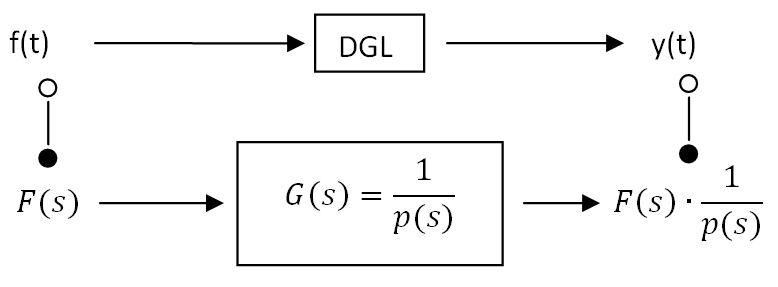
\includegraphics[width=14cm]{../IntTra/bilder/diffgleichungen.png}
				